% Atlas sample page: Breeding Grounds. Calligraphic adaptation. PROPOSAL, not canon.
% Canon text: Eusocial Interbeing/Ecology/Breeding Grounds.md at Zyphos 49207ef, verbatim.
% History: Meta Vens (created 1c5c14b, clarified 3700291); rename by MadmansLullabyOFFICIAL (3afb94f).
% Proposals: sample-breeding-grounds.proposal.md. Build: pdflatex sample-breeding-grounds.tex
% Wikilink brackets are dropped in the render; the words are the vault's.
% Hand: flowing chancery (psnfss `pzc`), the guess in design.md for Sa'ueia-side entries.
\documentclass[11pt,a4paper]{article}
\usepackage[T1]{fontenc}
\usepackage[utf8]{inputenc}
\usepackage[margin=24mm]{geometry}
\usepackage{xcolor,tikz,microtype,setspace}
\definecolor{ink}{HTML}{1F2A2A}
\definecolor{rubric}{HTML}{3F6B5E}
\definecolor{wash}{HTML}{ECEADF}
\newcommand{\hand}{\fontfamily{pzc}\selectfont}
\pagecolor{wash}\color{ink}
\pagestyle{empty}\setlength{\parindent}{0pt}\setlength{\parskip}{0.8em}
% A slot is a framed placeholder: nothing is rendered here.
\newcommand{\slot}[3]{%
  \begin{tikzpicture}
    \draw[rubric,line width=0.5pt] (0,0) rectangle (#1,#2);
    \draw[rubric,dashed] (0.06,0.06) rectangle (#1-0.06,#2-0.06);
    \node[text width=#1cm-1cm,align=center,font=\hand\small,text=rubric] at (#1/2,#2/2) {#3};
  \end{tikzpicture}}
\begin{document}
\begin{center}
{\hand\fontsize{34}{38}\selectfont\color{rubric} Breeding Grounds}\\[2mm]
{\hand\large Ecology\ \ $\cdot$\ \ the Sa'ueia continent}\\[1mm]
% Loose, wave-like rule: flowing hand for a Sa'ueia-side entry (guess).

\begin{tikzpicture}\draw[rubric,line width=0.6pt] plot[smooth,domain=0:10,samples=40] (\x,{0.08*sin(\x*180)});\end{tikzpicture}
\end{center}
\begin{center}\slot{15.5}{5.2}{PLATE (not rendered): a breeding ground. PR \#6 brief 10.}\end{center}
\onehalfspacing
{\hand\Large\color{rubric} B}{\hand\large reeding Grounds are sacred communal sites where the Sa'ueia breed and care for those who need to stay in one place. They remain occupied year-round, mainly by infants, infirm adults, caretakers, rotating specialists, and allied organisms.}

{\hand\large Most adults visit, then leave again with their family units. They return to breed, recover, teach, mourn, settle disputes, and renew obligations. The grounds provide shared places for reproduction and medical care, preserve communal memory, and anchor legal relationships. They also serve as places where important transitions are marked through ritual.}

{\hand\large These sites support a mobile civilization; they are not cities. If a breeding ground becomes a capital, the Sa'ueia system starts to break down. Concentrating the population permanently would invite hierarchy, exhaust resources, provoke ecological resentment, and leave the grounds vulnerable to imperial-style capture.}

\vfill
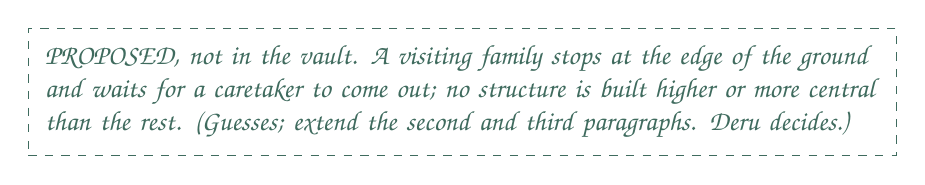
\begin{tikzpicture}
\node[draw=rubric,dashed,text width=10.6cm,inner sep=6pt,font=\hand\normalsize,text=rubric]
{\textbf{PROPOSED, not in the vault.} A visiting family stops at the edge of the ground and waits for a caretaker to come out; no structure is built higher or more central than the rest. (Guesses; extend the second and third paragraphs. Deru decides.)};
\end{tikzpicture}\hfill\slot{4}{2.6}{SPOT: route-memory instrument (PR \#6 brief 11)}

\vspace{4mm}
{\hand\small Source: Zyphos \texttt{Eusocial Interbeing/Ecology/Breeding Grounds.md}, commit 49207ef. Text by Meta Vens; only the wikilink brackets are dropped.}
\end{document}
